\documentclass[unicode,12pt]{beamer}
\usetheme[progressbar=frametitle]{metropolis}    %プレゼンのテーマ設定

%if want to use pdfLatex, specify \iffalse to preamble for LuaLatex and XeLatex
%--------------- preamble for LuaLatex ------------------%

\iffalse
\usepackage{luatexja}
\usepackage[ipaex]{luatexja-preset}
\renewcommand{\kanjifamilydefault}{\gtdefault}
\setsansfont{Calibri}
\fi

%-----------------------------------------------------%

%--------------- preamble for XeLatex -------------------%

\iftrue
\usepackage{xltxtra}
\XeTeXlinebreaklocale "ja"
\usepackage{zxjatype}
\setCJKmainfont[]{Meiryo}
\setsansfont[Scale = 1.1]{Calibri}  % or Arial (Scale = 1)
\fi

%-----------------------------------------------------%

%--------------- general preamble -----------------------%

\definecolor{Cerulean blue}{rgb}{0.16, 0.32, 0.75}
\definecolor{darkcerulean}{rgb}{0.03, 0.27, 0.49}
\definecolor{skyblue}{rgb}{0.4, 0.6, 1.0}
\definecolor{lightpink}{rgb}{1.0, 0.8, 0.76}  %for block color
\definecolor{gray}{gray}{0.8}

\setbeamertemplate{blocks}[default] % Blockの影を消す
%\setbeamertemplate{items}[default] % 箇条書きをシンプルに
\setbeamertemplate{navigation symbols}{} % ナビゲーションシンボルを消す
\setbeamertemplate{footline}[frame number] % フッターはスライド番号のみ
\setbeamertemplate{itemize item}[circle]
\setbeamertemplate{itemize subitem}{--}
\setbeamercolor{frametitle}{bg=skyblue} %or Cerulean blue
\setbeamercolor{title}{fg=darkcerulean}

\iffalse
\usebackgroundtemplate{
    \includegraphics[width=\paperwidth,height=\paperheight]{beamer_background1.pdf}
}
\fi

\usepackage{color}
\usepackage{graphicx}
\graphicspath{{_images/}{../_images/}}


\newcommand{\emphasis}[2][red]{{\bf{\color{#1} #2}}}
\newcommand{\caveat}[2][blue]{{\bf{\color{#1} #2}}}
\newcommand{\fpartial}[3][\partial]{\frac{#1 #2}{#1 #3}}
\newcommand{\hpartial}[4][\partial]{\frac{#1^{#2} #3}{#1 #4^{#2}}}

\newcommand{\dlinecell}[1]{\begin{tabular}{@{}c@{}} #1 \end{tabular}}

\def\argmax{\text{arg} \max}
\def\argmin{\text{arg} \min}

%-----------------------------------------------------%

\title{Status Goods: Experimental evidence from platinum credit cards}
\subtitle{Bursztyn, Ferman, Fiorin, Kanz, and Rao (2018, QJE)}
\author{Hiroki Kato}
\date{October 29, 2020 (OS seminar)}

\begin{document}

    \maketitle

    \iffalse
    \begin{frame}
        \frametitle{Conspicuous Consumption}
    
        \begin{quote}
            日常生活における冷淡な観察者たちに、自らの金銭的能力を見せつけるために利用しうる唯一の手段は、たえず支払能力を見せつけることである(ソースティン・ヴェブレン「有閑階級の理論」)
        \end{quote}

        \centerline{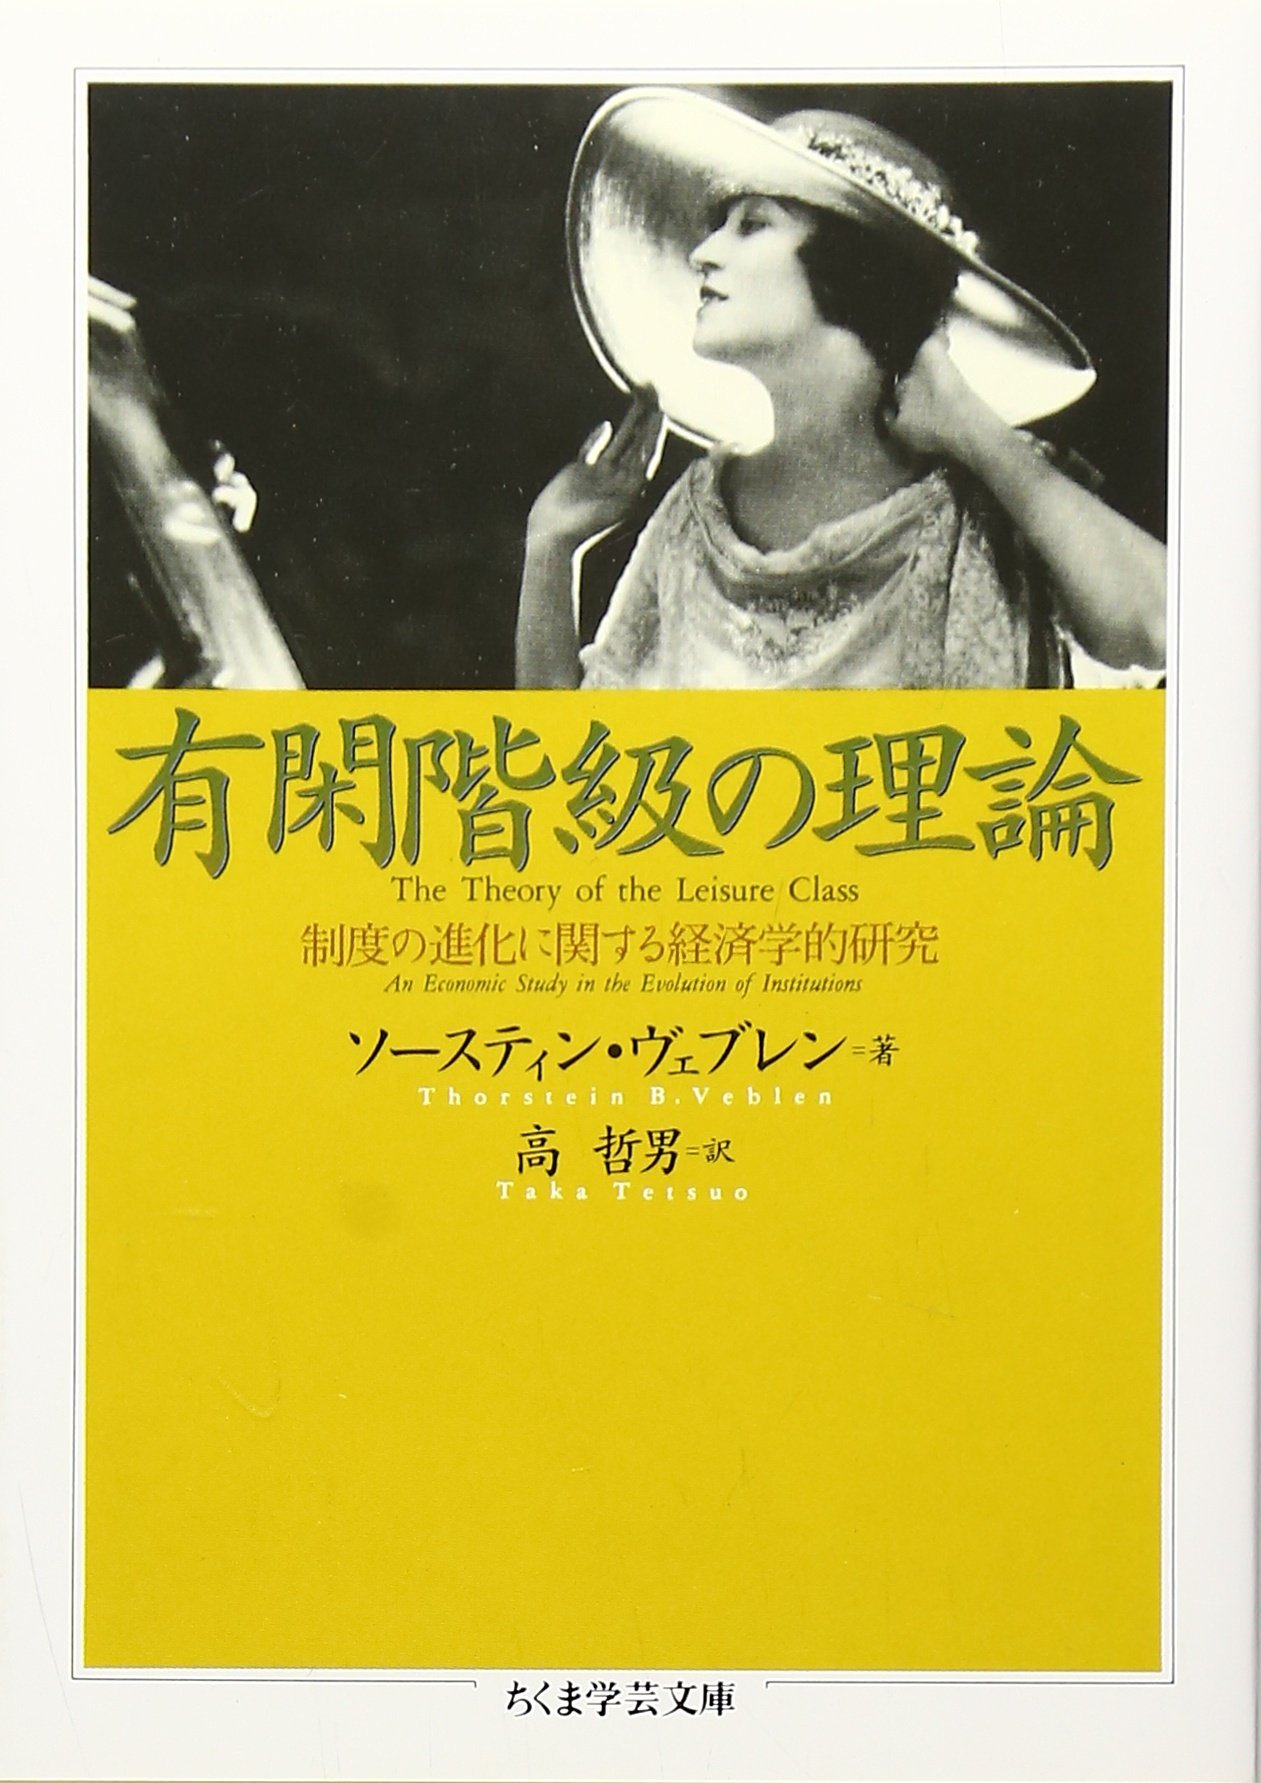
\includegraphics[width = 0.25\linewidth]{0717kato/veblen.jpg}}
    
    \end{frame}
    \fi

    \begin{frame}
        \frametitle{Social Image and Consumption}
    
        \begin{itemize}
            \item Consumption may be shaped by social image concerns.
            \item A desire to signal high income or wealth cause consumers to purchase status goods (conspicuous consumption)
            \item As the status good becomes accessible to lower-income consumers, this weakens its income-signaling power and promotes higher-income consumers to demand a more exclusive status good (positional externalities).
        \end{itemize}
    
    \end{frame}

    \begin{frame}
        \frametitle{Difficulty and Open Question}
    
        \begin{itemize}
            \item With observational data, it is difficult to separate unobserved consumption utility from a desire to signal high income.
            \item Self-image (self-esteem, identity) and the demand for status could be deeply connected, and it remains an open question whether self- and social image are substitutes or complements.
        \end{itemize}
    
    \end{frame}

    \begin{frame}
        \frametitle{What This Paper Studied}
    
        This paper (i) provides two field-experimental evidence of the existence of status goods and its associated positional externalities; and (iii) provide an on-line experiment evidence of substitution between self- and social image.
        \begin{itemize}
            \item Authors work with a large bank in Indonesia to design two related experiments and one observational study that market the bank's widely recognized platinum credit cards.
            \item Additionally, authors conduct one on-line experiment via MTurk.
        \end{itemize}
    
    \end{frame}

    \section{Background of Credit Cards}

    \begin{frame}
        \frametitle{Characteristics of Credit Cards}
    
        \begin{itemize}
            \item The bank offers its credit card product in three tires: classic, gold, and platinum.
            \begin{itemize}
                \item The three tiers are vertically differenciated based on income.
                \item Only 10\% qualify for a platinum card, 72\% have a gold card, and 18\% qualify only for the classic card.
                \item The bottom quartile of the customer is close to the median income of urban Indonesia, while the median credit card customer is in the top 15\% of urban incomes in Indonesia.
            \end{itemize}
        \end{itemize}
    
    \end{frame}

    \begin{frame}
        \frametitle{Design of Credit Cards}

        The platinum card differs from the two lower-tier cards in both color and design.
    
        \centerline{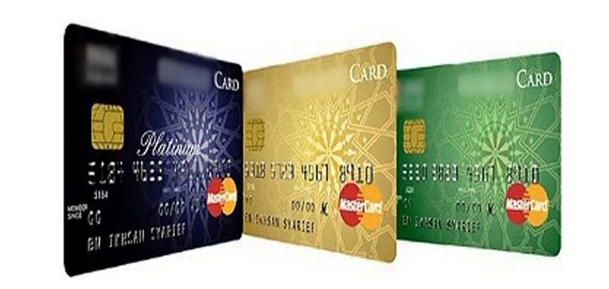
\includegraphics[width = \linewidth]{0717kato/creca.PNG}}
    
    \end{frame}

    \begin{frame}
        \frametitle{Public Recognition of Platinum Card}
    
        \begin{itemize}
            \item This paper sees the platinum card as a status good.
            \item A necessary condition for status signaling is public Recognition of the platinum card.
            \item To test it, authors conducted two surveys outside malls in the greater Jakarta area.
            \begin{itemize}
                \item First survey (N = 113): 93 respondents ranked the cards correctly in terms of their income requirements.
                \item Second survey (N = 500): 59\% recognized the platinum card as having a higher income criterion. Restricting those who have a credit card, this share increases to 71\%
            \end{itemize}
        \end{itemize}
    
    \end{frame}

    \section{Experiment 1: Demand For the Platinum Card vs Its Instrumental Benefits}


    \begin{frame}
        \frametitle{Goal and Sample}
    
        \begin{itemize}
            \item Goal: to test whether part of the demand for the platinum card is unrelated to its instrumental features
            \item Sample: 1,260 customers randomly drawn from the set of current gold card holders with relatively high income. These were customers to whom the bank was willing to offer an upgrade to the platinum card, even though they may not have normally qualified for it.
            \item Outcome: The take-up rate of the platinum card by marketing calls.
        \end{itemize}
    
    \end{frame}

    \begin{frame}
        \frametitle{Treatment}
    
        \begin{enumerate}
            \item \textit{Platinum upgrade treatment}: customers were offered an upgrade the the bank's regular platinum card.
            \item \textit{Benefits upgrade treatment}: customers were offered the same services as the platinum card, but as an add-on their current gold card.
            \item \textit{Platinum upgrade merit treatment}: Instead of being told they were randomly chosen, they were told, ``As one of our top customers, you have been chosen to receive an upgrade to our platinum card.''
        \end{enumerate}
         
    \end{frame}

    \begin{frame}
        \frametitle{Hypothesis}
    
        Platinum upgrade vs. Benefits upgrade
        \begin{itemize}
            \item Difference between treatments: card appearance
            \item Hypothesis: Platinum upgrade > Benefits upgrade if the platinum card is a status good.
        \end{itemize}
        Platinum upgrade vs. Platinum upgrade merit 
        \begin{itemize}
            \item Difference between treatments: reason of selection
            \item Hypothesis: Platinum upgrade merit $\not=$ Platinum upgrade if the demand of status good depends on self-image.
        \end{itemize}
    
    \end{frame}

    \begin{frame}
        \frametitle{Implementaion}
    
        \begin{itemize}
            \item Implementation: 
            \begin{itemize}
                \item The experiment was conducted over the course of one week.
                \item Each client received the offer only once, but up to three call attempts were made if a client could not be reached
                \item No additional calls were made once any part of the offer had been revealed to a respondent.
                \item The callers were able to reach 835 out of 1260 clients.
            \end{itemize}
        \end{itemize}
    
    \end{frame}

    \begin{frame}
        \frametitle{Results}
    
        \centerline{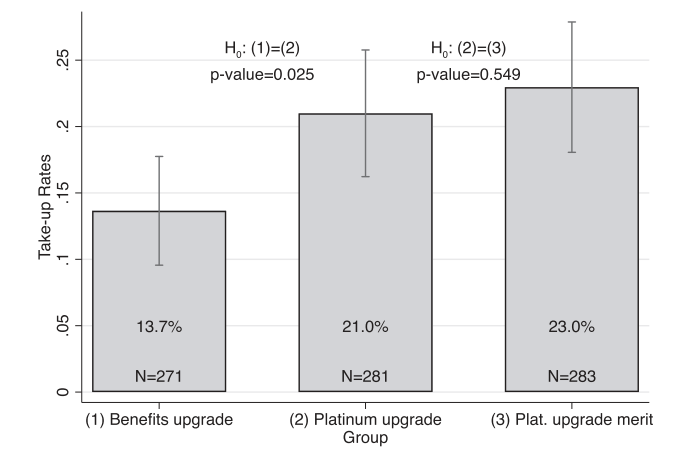
\includegraphics[width = \linewidth]{0717kato/result_exp1.PNG}}
    
    \end{frame}

    \begin{frame}
        \frametitle{Interpretaions of Result}
    
        \begin{itemize}
            \item Benefits upgrade vs. Platinum upgrade
            \begin{itemize}
                \item Strong demand for the physical appearance of the new card the customers receive.
            \end{itemize}
            \item Plat. upgrade merit vs. Platinum upgrade
            \begin{itemize}
                \item Self-image may not affect the demand for status. The merit treatment was too weak to stimulate self-image.
                \item Informing customers they had been randomly chosen to receive the platinum offer was not perceived as off-putting or particularly unnatural.
            \end{itemize} 
        \end{itemize}
    
    \end{frame}

    \begin{frame}
        \frametitle{Remarks}
    
        \begin{itemize}
            \item The bank made a second call to customers who had declined the offer and offered them the same upgrade at a 25\% discount. This increased demand for the benefits upgrade by only 3.7\% points.
            \item One potential confounding is customer suspicion. This is not serious because only 1\% of the respondents stated that they had doubts that the quality of the benefits and services would be identical to the platinum card.
        \end{itemize}
        
    \end{frame}

    \section{Observational Study: Status Signaling in Credit Card Transaction Data}

    \begin{frame}
        \frametitle{Goal and Data}
    
        \begin{itemize}
            \item Goal: To test whether platinum card holders are more likely to use the card than gold card holders in the social settings.
            \item Data: Credit card transaction data for customers with active credit cards who opened their accounts between January 2014 and August 2015, and who have gold card with Rp 20 million or Rp 30 million credit limits (the highest credit limit) or platinum card with Rp 40 million and Rp 50 million credit limit (the lowest credit limit).            
        \end{itemize}
    
    \end{frame}

    \begin{frame}
        \frametitle{Category of Transactions}
    
        \begin{itemize}
            \item \textit{visible} transaction: restaurants, cafes, and bars (89\%), in membership clubs (2\%), movie theaters (2\%), and other amusement and recreational services (7\%)
            \item \textit{online} transaction: transactions with internet-related terms, such as ``www,'' ``.com'', or ``e-store,'' in the text description
            \item \textit{retail} transaction: supermarkets, grocery and convenience stores (30\%), department stores (10\%), service stations (7\%), clothing stores (6\%), and at other merchants, such as pharmacies (47\%).
        \end{itemize}
    
    \end{frame}

    \begin{frame}
        \frametitle{Empirical Strategy}
    
        \begin{itemize}      
            \item Outcome: The share of visible transaction    
            \item Variation in credit limits as a proxy for income and creditworthiness.
            \begin{itemize}
                \item Main: compare the lowest-income platinum card holders (Rp 40 million credit limit) with the highest-income gold card holders (Rp 30 million credit limit).
                \item Ruling out credit limit: compare within the platinum card group (Rp 40 million versus Rp 50 million credit limit) and within the gold card group (Rp 20 million versus Rp 30 million credit limit)
            \end{itemize}
        \end{itemize}
    
    \end{frame}

    \begin{frame}
        \frametitle{Results}
    
        \centerline{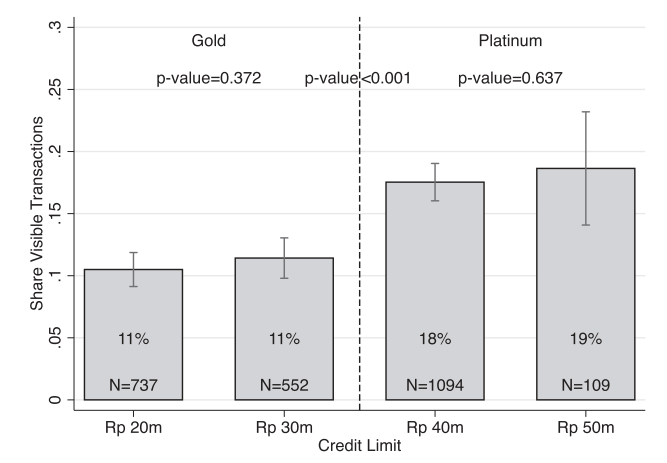
\includegraphics[width = \linewidth]{0717kato/result_obs.PNG}}
    
    \end{frame}

    \begin{frame}
        \frametitle{Results}
    
        \centerline{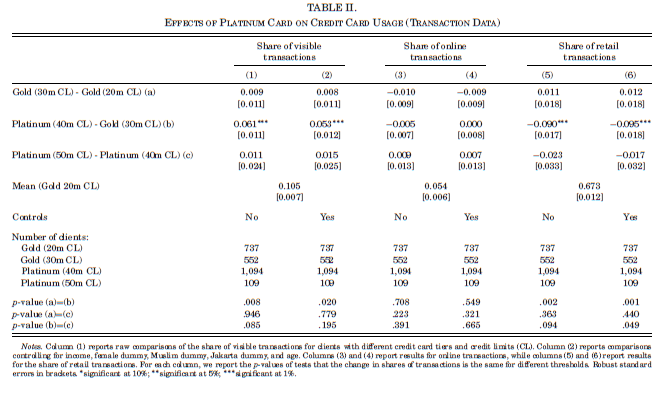
\includegraphics[width = \linewidth]{0717kato/result_obs2.PNG}}
    
    \end{frame}

    \begin{frame}
        \frametitle{Interpretaion}
    
        \begin{itemize}
            \item Platinum card holders use their card to signal income to their peers in social settings.
            \begin{itemize}
                \item The main difference is not simply related to a credit limit increase. 
            \end{itemize}
            \item There is not significant change in the share of online transactions between the gold card with Rp 30m and the platinum card with Rp 40m, and a significant decrease in the proportion of retail transactions.
        \end{itemize}
    
    \end{frame}

    \begin{frame}
        \frametitle{Mechanism}
    
        \begin{itemize}
            \item Having a platinum card does not make customers more likely to go to restaurants. However, they use different modes of payment for these restaurant expenditures.
            \item No price effects since the platinum card does not offer cash back in restaurants. 48\% of platinum card holders own other credit cards that offer cash back.  
            \item Platinum card holders therefore appear willing to pay a cost to show off their card, forgoing cash back from other credit cards (a costly signal).
        \end{itemize}
        
    \end{frame}

    \section{Experiment 2: Positional Externality}

    \begin{frame}
        \frametitle{Goal}
    
        Goal: to show negative positional externality
        \begin{itemize}
            \item When individuals with comparatively lower social status gain access to a status good, it diminishes its signaling value and imposes a negative positional externality on the current owners of the status good. This, in turn, should induce the earliest adopters to demand a more exclusive status good.
        \end{itemize}
    
    \end{frame}

    \begin{frame}
        \frametitle{Background and Sample}
    
        \begin{itemize}
            \item Background: A few months prior to this experiment, the bank had reduced the income threshold necessary to qualify for a platinum card and was considering the incroduction of a new credit card tier above platinum (diamond card) reserved for its highest-income customers.
            \item Sample: 180 platinum card customers, who joined under the old income requirement and were unaware of the recent change in the platinum credit card's income eligibility.
        \end{itemize}
    
    \end{frame}

    \begin{frame}
        \frametitle{Treatment}
    
        \begin{itemize}
            \item Treatment: A costly take-up experiment in which they offered the diamond card, which is a new credit card tier above platinum.
            \begin{itemize}
                \item \textit{Control}: The caller explained that the diamond card would have the exact same services, benefits, credit limit, and additional services as the platinum card, but would differ in color and design.
                \item \textit{Positional externality treatment}: Additional information that the bank had recently relaxed the eligibility criteria for the platinum card
            \end{itemize}
        \end{itemize}
    
    \end{frame}

    \begin{frame}
        \frametitle{Results}
    
        \centerline{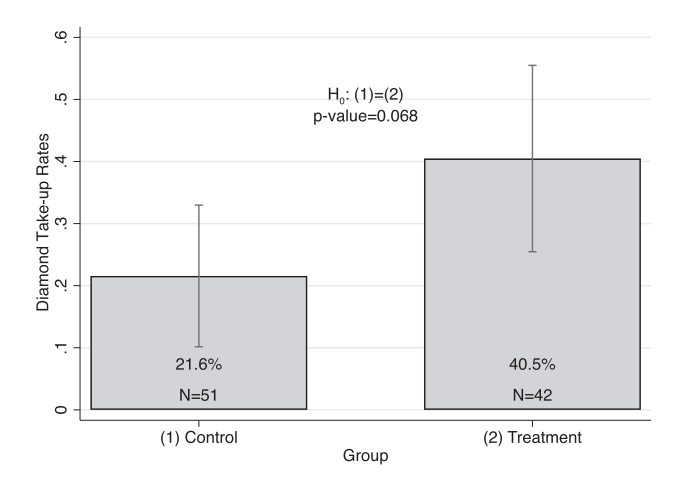
\includegraphics[width = \linewidth]{0717kato/result_exp2.PNG}}
    
    \end{frame}

    \begin{frame}
        \frametitle{Interpretaion}
    
        \begin{itemize}
            \item Demand for the diamond card increases when customers are informed that the platinum card is now available to a wider group of customers.
            \begin{itemize}
                \item This statistical significance increases when controlling for baseline covariates.
            \end{itemize}
            \item As lower-status consumers begin adopting the status good, they cause higher-status consumers to demand more exclusive products.
        \end{itemize}
    
    \end{frame}

    \section{MTurk Experiment: Self-Image and Status Goods}

    \begin{frame}
        \frametitle{Goal and Sample}
    
        \begin{itemize}
            \item Goal: to test whether high self-esteem, which is an important component of self-image, affects the demand for status goods
            \begin{itemize}
                \item high-income individuals might demand status goods because they derive utility from making consumption choices consistent with their self-image, irrespective of the social visibility of their consumption. 
            \end{itemize}
            \item Sample: 405 individuals who signed up for an incentivized task on the online platform MTurk in August 2016.
        \end{itemize}
    
    \end{frame}

    \begin{frame}
        \frametitle{Experimental Protocol}
    
        \begin{enumerate}
            \item Randomized tasks
            \begin{itemize}
                \item \textit{treatment}: to write a paragraph about a recent experience or achievement that made them proud (self-affirmation exercise)
                \item \textit{control}: to write the title and summarize the story of the last movie you have seen
            \end{itemize}
            \item Incentivized choices of a lottery in which they can win either gift certificates for a luxury apparel (Armani) or for a non-luxury apparel (Old Navy).
            \begin{itemize}
                \item US\$500 for Old Navy or US\$400 (\$450, \$500, \$550, \$600) for Armani
            \end{itemize}
            \item rank the values they consider importance of life (self-esteem score).
        \end{enumerate}
    
    \end{frame}

    \begin{frame}
        \frametitle{Results}
    
        \centerline{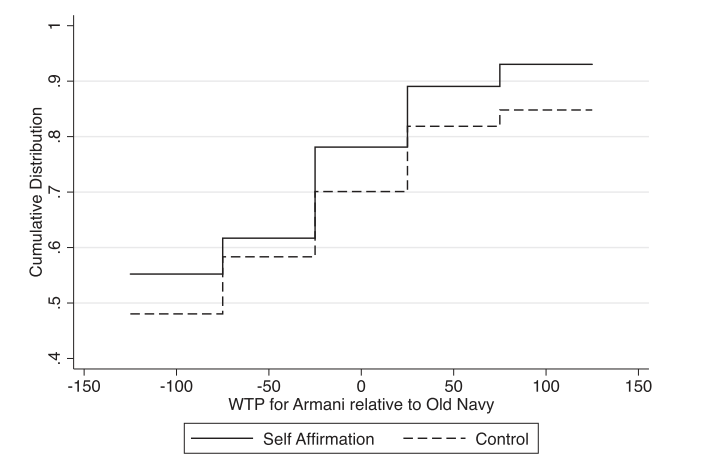
\includegraphics[width = \linewidth]{0717kato/result_exp3.PNG}}
    
    \end{frame}

    \begin{frame}
        \frametitle{Regression Results}
    
        \centerline{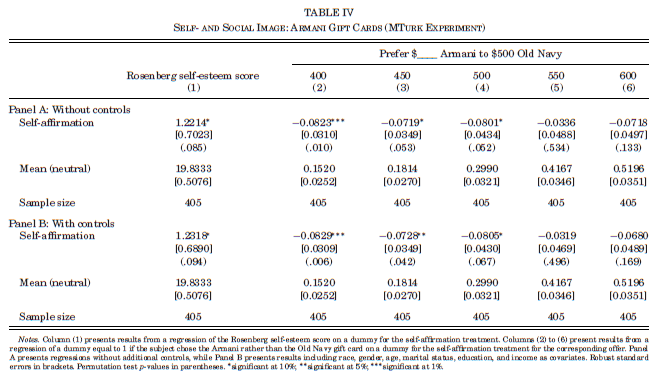
\includegraphics[width = \linewidth]{0717kato/result_exp32.PNG}}
    
    \end{frame}

    \begin{frame}
        \frametitle{Interpretaion}
    
        \begin{itemize}
            \item Self-affirmation treatment icreases subjects' self-esteem score. The treatment succeeded in stimulating self-esteem.
            \item The self-affirmation treatment has a negative effect on the willingness to pay for the Armani gift card.
            \item Higher self-image reduces individuals' desire for social image, and thus their demand for status goods. That is, self- and social image are substitutes.
        \end{itemize}
    
    \end{frame}

    \section{Conclusions}

    \begin{frame}
        \frametitle{Conclusions}
    
        This paper shows the status aspect of a platinum credit card
        \begin{itemize}
            \item the demand for card is mainly driven by its status aspect rather than its instrumental benefit 
            \item the demand for a higher credit card increases when the income threshold of a platinum card becomes lower.
        \end{itemize}
        Also, this paper provides suggestive evidence that higher self-esteem causally reduces demand for status goods.
    
    \end{frame}




\end{document}